%%%%%%%%%%%%%%%%%%%%%%%%%%%%%%%%%%%%%%
  %%%%%%%%%%%%%%%%%%%%%%%%%%%%%%%%%%%%%%
  % Do not edit the TeX file your work
% will be overwritten.  Edit the RnW
% file instead.
%%%%%%%%%%%%%%%%%%%%%%%%%%%%%%%%%%%%%%
  %%%%%%%%%%%%%%%%%%%%%%%%%%%%%%%%%%%%%%
  

      

\begin{knitrout}
\definecolor{shadecolor}{rgb}{0.969, 0.969, 0.969}\color{fgcolor}\begin{figure}[!h]

{\centering 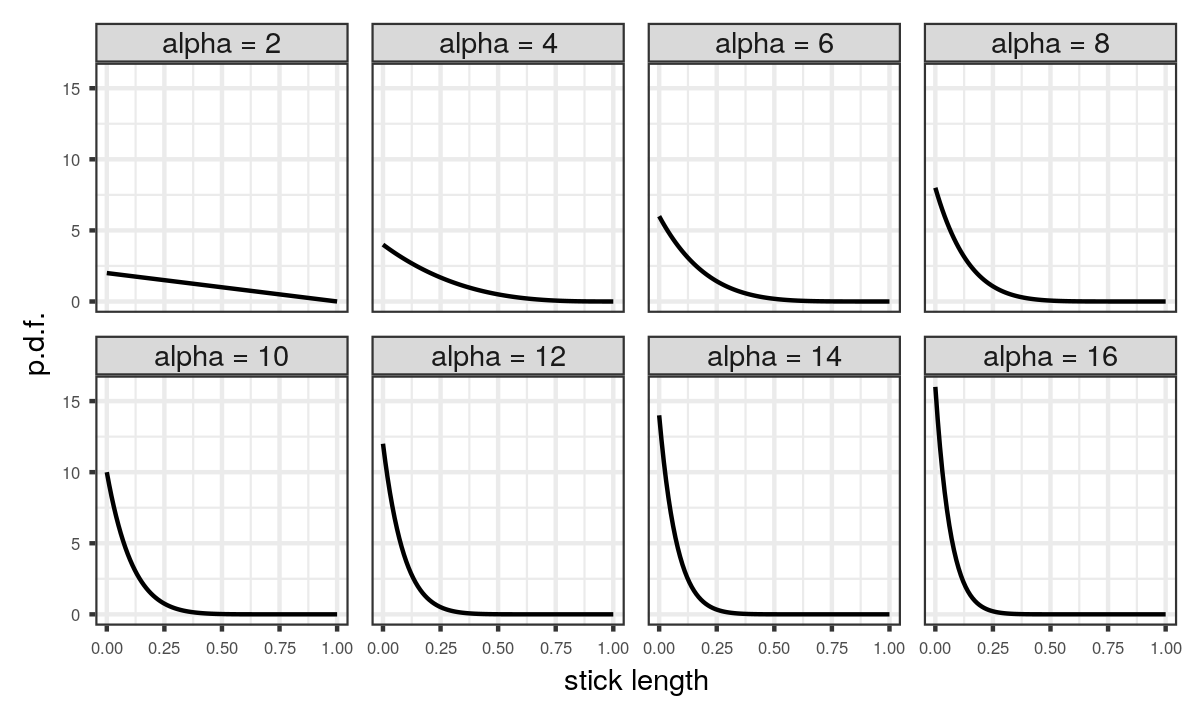
\includegraphics[width=0.980\linewidth,height=0.588\linewidth]{figure/beta_priors-1} 

}

\caption[Probability density functions of $\text{Beta}(1, \alpha)$ distributions, for various $\alpha$]{Probability density functions of $\text{Beta}(1, \alpha)$ distributions, for various $\alpha$. }\label{fig:beta_priors}
\end{figure}


\end{knitrout}

      

\begin{knitrout}
\definecolor{shadecolor}{rgb}{0.969, 0.969, 0.969}\color{fgcolor}\begin{figure}[!h]

{\centering 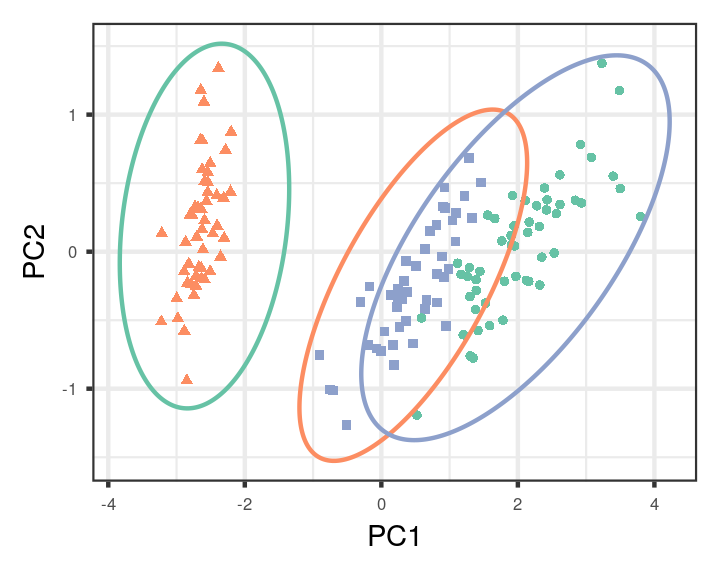
\includegraphics[width=0.588\linewidth,height=0.470\linewidth]{figure/iris_fit-1} 

}

\caption[The iris data in principal component space and 
                      GMM fit at $\alpha = 6$]{The iris data in principal component space and 
                      GMM fit at $\alpha = 6$. 
                      Colors denote inferred memberships and
                      ellipses are estimated covariances. }\label{fig:iris_fit}
\end{figure}


\end{knitrout}


\begin{knitrout}
\definecolor{shadecolor}{rgb}{0.969, 0.969, 0.969}\color{fgcolor}\begin{figure}[!h]

{\centering 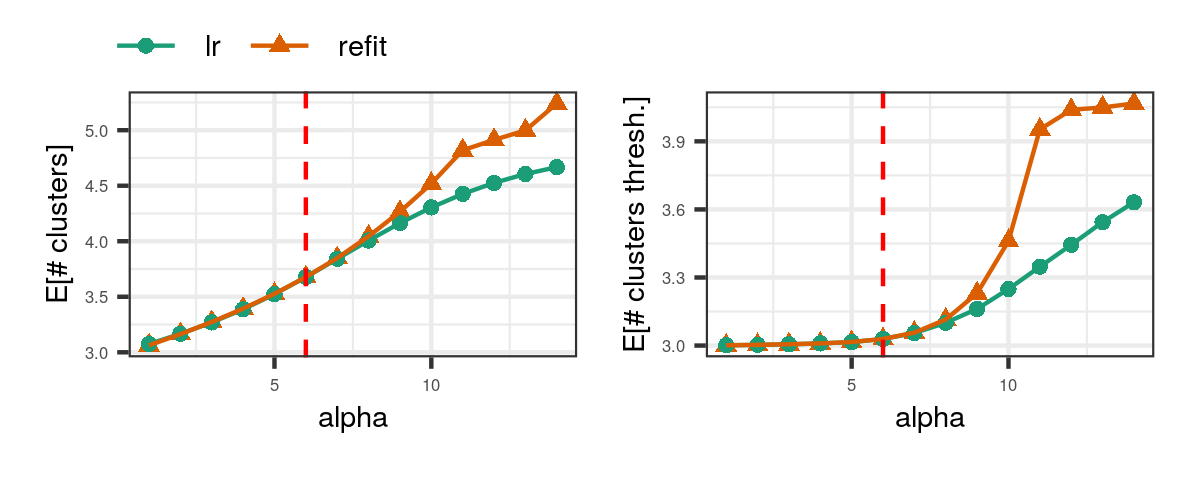
\includegraphics[width=0.980\linewidth,height=0.392\linewidth]{figure/iris_alpha_sens-1} 

}

\caption[The expected number of posterior predictive clusters in the iris data as $\alpha$ varies]{The expected number of posterior predictive clusters in the iris data as $\alpha$ varies. 
We compute the linear approximation at $\alpha=6$ and
extrapolate the expected number of clusters using the
linear approximation (green).
We compare against the expected number of clusters obtained by refitting the model at each $\alpha$ (orange). In the right plot, the threshold was set at $t = 5$. }\label{fig:iris_alpha_sens}
\end{figure}


\end{knitrout}



\begin{knitrout}
\definecolor{shadecolor}{rgb}{0.969, 0.969, 0.969}\color{fgcolor}\begin{figure}[!h]

{\centering 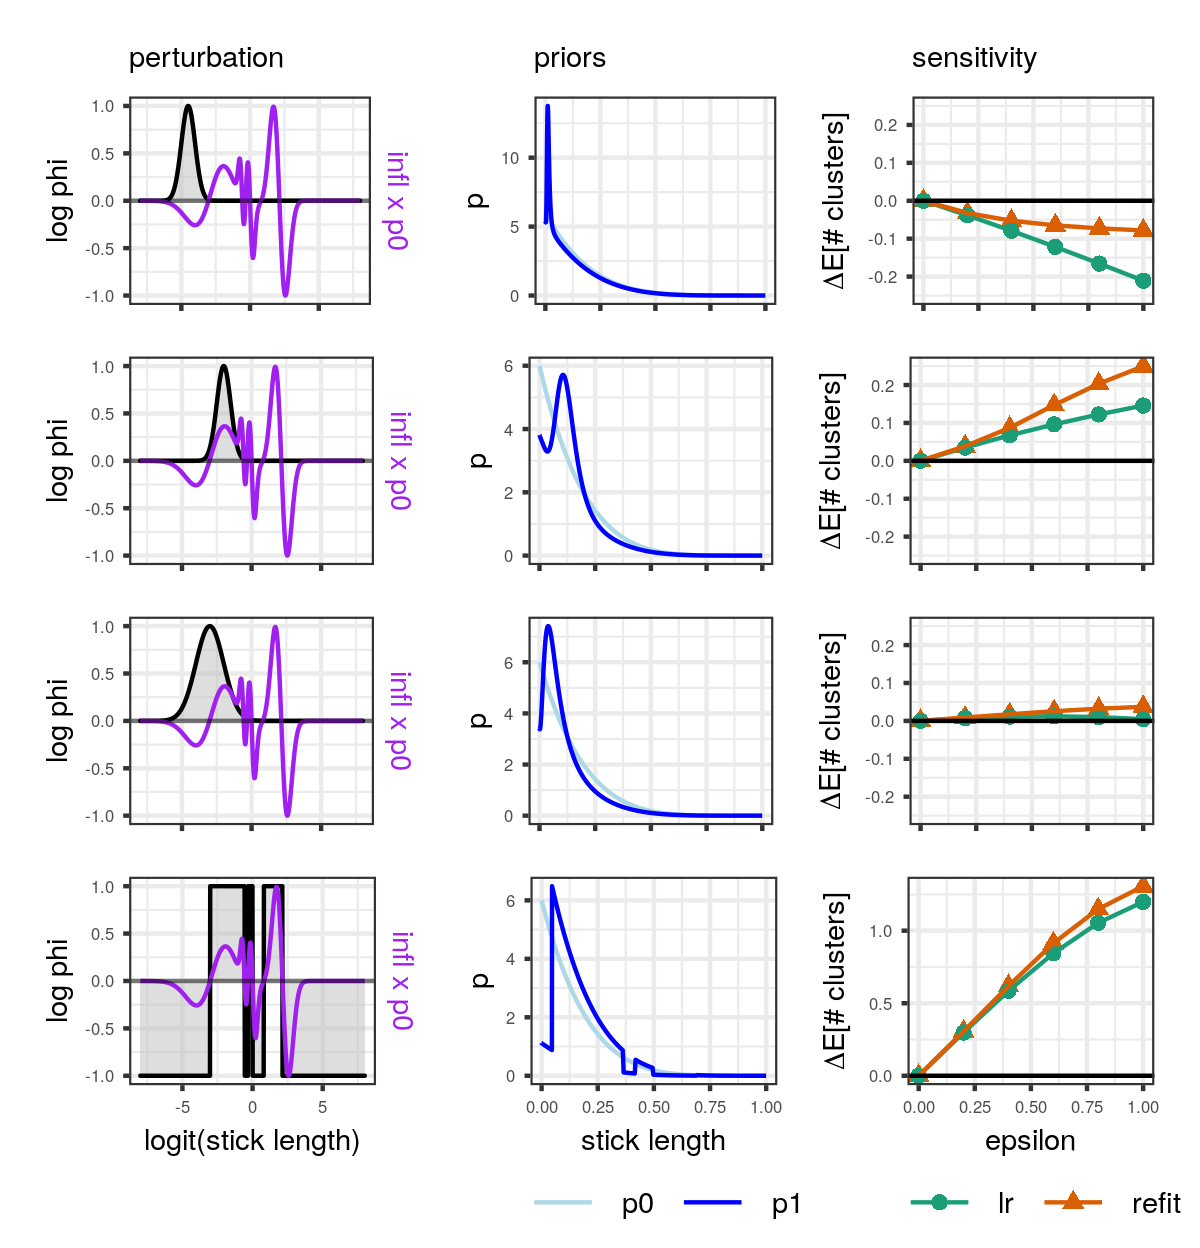
\includegraphics[width=0.980\linewidth,height=1.019\linewidth]{figure/iris_fsens-1} 

}

\caption{Sensitivity of
        the expected number of posterior predictive clusters in the iris dataset
        to four multiplicative perturbations with 
        $L_{\infty}$-norm equal to one. 
        (Left) The log multiplicative perturbation $\log\phi$ in grey.        
        In purple is the prior-weighted influence function, scaled to also have 
        unit $L_{\infty}$-norm. 
        (Middle) The original prior density $p_0$ and 
        the perturbed prior density $p_1 = p_0\times \phi$. 
        (Right) The effect of the perturbation 
        on the change in expected number of clusters as a function of $\epsilon$. }\label{fig:iris_fsens}
\end{figure}


\end{knitrout}


